\chapter{TANGENTIAL CUTTER}


\section{General Information}

A tangential cutter is a type of cutting tool commonly used in CNC machining
for cutting materials such as vinyl, fabric, foam, and other thin or flexible materials.
Unlike traditional rotary cutters that rotate about a central axis,
tangential cutters have a cutting edge that moves tangentially to the material being cut.

\begin{figure}[h!tb]
\centering
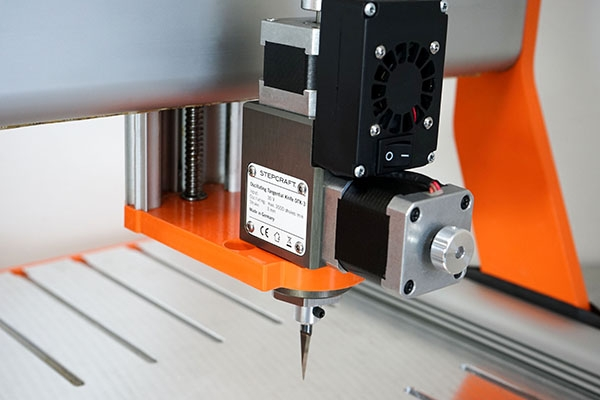
\includegraphics[scale=0.80]{otc.jpg}
\caption{A Tangential Cutter}
\label{fig:label3}
\end{figure}


Here's some information about tangential cutters.

\noindent\textbf{Principle of Operation.}
Tangential cutters work by moving the cutting edge along a linear path, perpendicular to the material surface, while maintaining a fixed orientation relative to the material.
This allows for precise and controlled cutting of intricate shapes and patterns, particularly in thin or flexible materials that may be prone to tearing or distortion with traditional rotary cutters.

\noindent\textbf{Design.}
Tangential cutters typically consist of a blade or cutting tip mounted on a mechanism that allows for precise control of the cutting angle and depth.
The cutting edge may be a straight blade, a beveled blade, or a specialized cutting tip depending on the application and material being cut.
The cutter is attached to a CNC machine's tool holder and is controlled by the machine's software to follow the desired cutting path.

\noindent\textbf{Applications.}
Tangential cutters are commonly used in applications such as sign making, textile cutting, gasket fabrication, packaging, and prototyping.
They are particularly well-suited for cutting intricate designs, small details, and sharp corners in materials that may be difficult to cut with traditional rotary cutters.

\noindent\textbf{Versatility.}
Tangential cutters can be used with a wide range of materials, including vinyl, fabric, leather, foam, paper, cardboard, and more.
They are capable of cutting both straight lines and complex curves with high precision and repeatability.

\noindent\textbf{Software Control.}
Tangential cutters are typically controlled by CNC software that generates toolpaths based on the desired cutting pattern or design.
The software calculates the optimal path for the cutter to follow, taking into account factors such as cutting speed, depth of cut, and corner handling to achieve the desired cut quality and accuracy.

\noindent\textbf{Advantages.}
Tangential cutters offer several advantages over traditional rotary cutters, including greater precision, reduced material waste, improved cut quality, and the ability to cut thicker or more rigid materials without distortion.
They are also capable of cutting small features and sharp corners with high accuracy.

Overall, tangential cutters are versatile and precise cutting tools commonly used in CNC machining for cutting a wide range of materials with high accuracy and repeatability.
Their ability to cut intricate designs and handle thin or flexible materials makes them valuable tools in various industries and applications.

\section{Transforming a 3D Printer into a Tangential Cutter}

To transform a FDM 3D Printer,
we reposition the extruder stepper motor in such a way that
we can attach a blade on the shaft of the stepper motor and revolve it at given angles.
To this end, we used a mont as given in the following graphic.

%{\Huge !!!Insert Graphic - Blade Mount!!!}

\begin{figure}[h!tb]
\centering
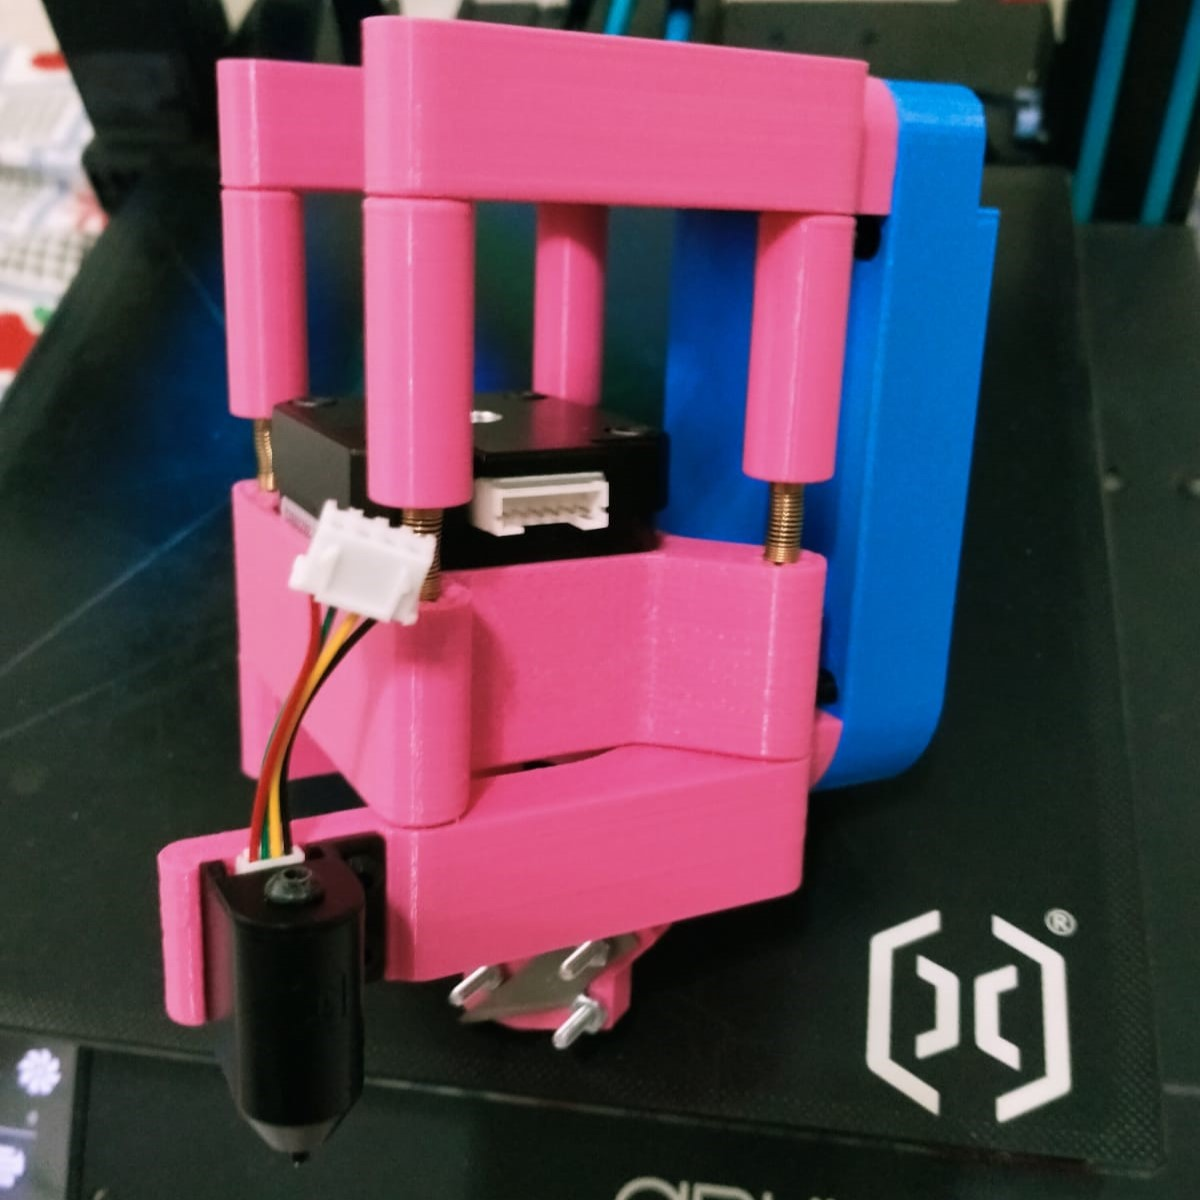
\includegraphics[scale=0.30]{tc-3.jpg}
%\rule{50mm}{50mm}
\caption{Tangential Cutter - Blade Mount}
\label{fig:label4}
\end{figure}


%{\Huge !!!Insert Graphic - Tangential Cutter!!!}

\begin{figure}[h!tb]
\centering
%\rule{50mm}{50mm}
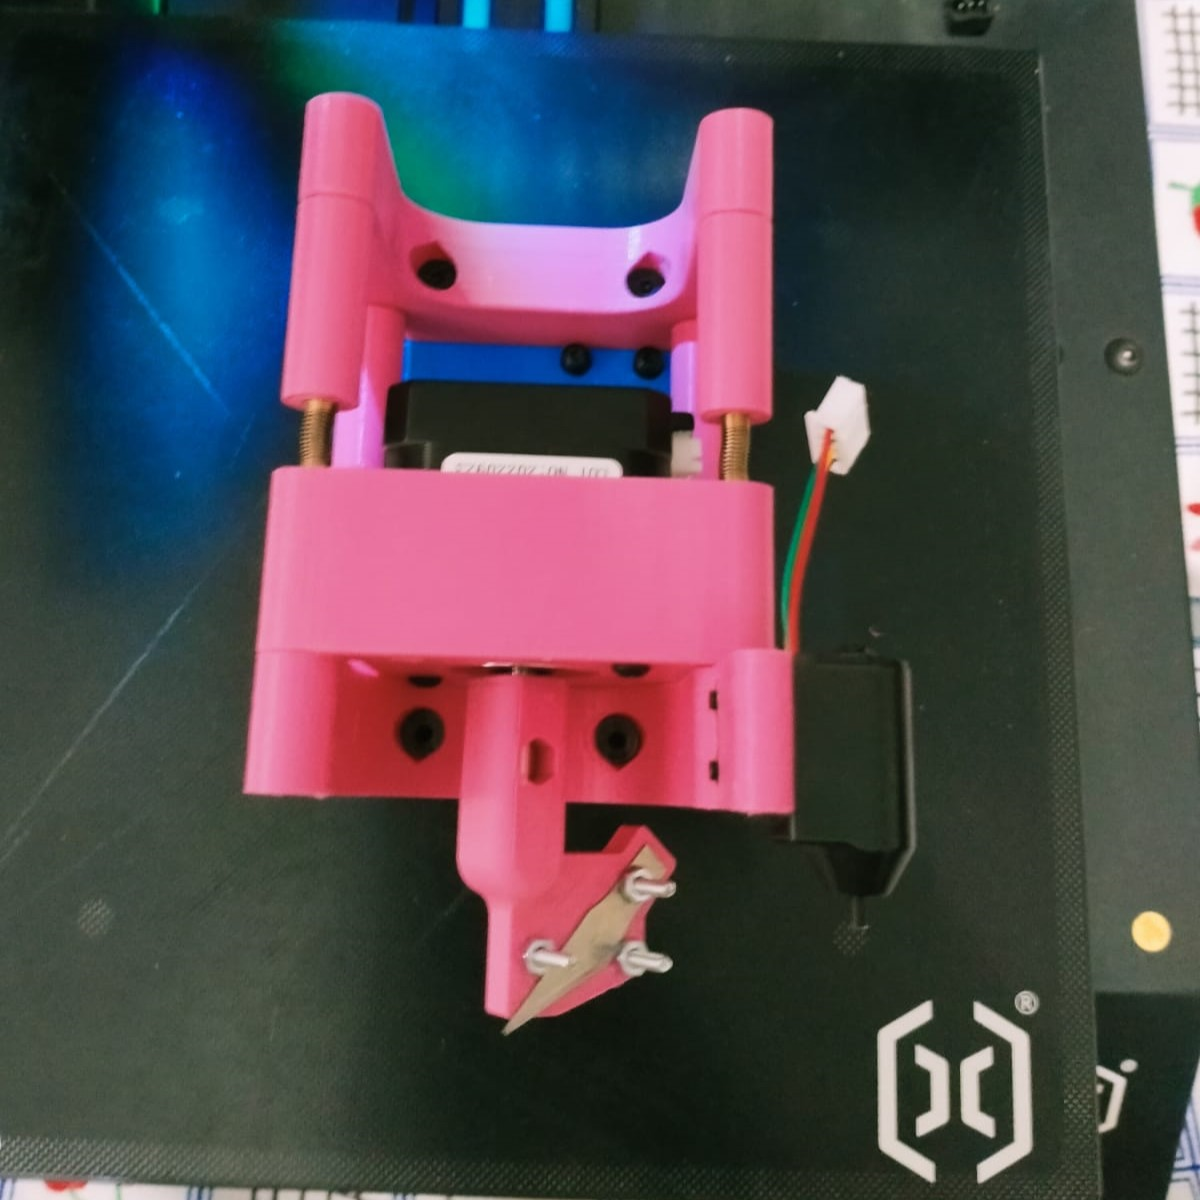
\includegraphics[scale=0.30]{tc-4.jpg}
\caption{Artillery Sidewinder X2 Modified as a Tangential Cutter}
\label{fig:label5}
\end{figure} 